% file: reasoning_case.tex

\begin{ReasoningBox}[title=Pattern Recognition] % 可以通过 title 参数修改标题
    % --- 第一部分：问题描述与图片 ---
    % \begin{minipage}[t]{0.58\textwidth}
    \begin{wrapfigure}{r}{0.3\textwidth}
        \centering
        % wrapfigure 通常顶部会有多余空白，使用负 vspace 向上提，让图片和第一行文字对齐
        \vspace{-20pt} 
        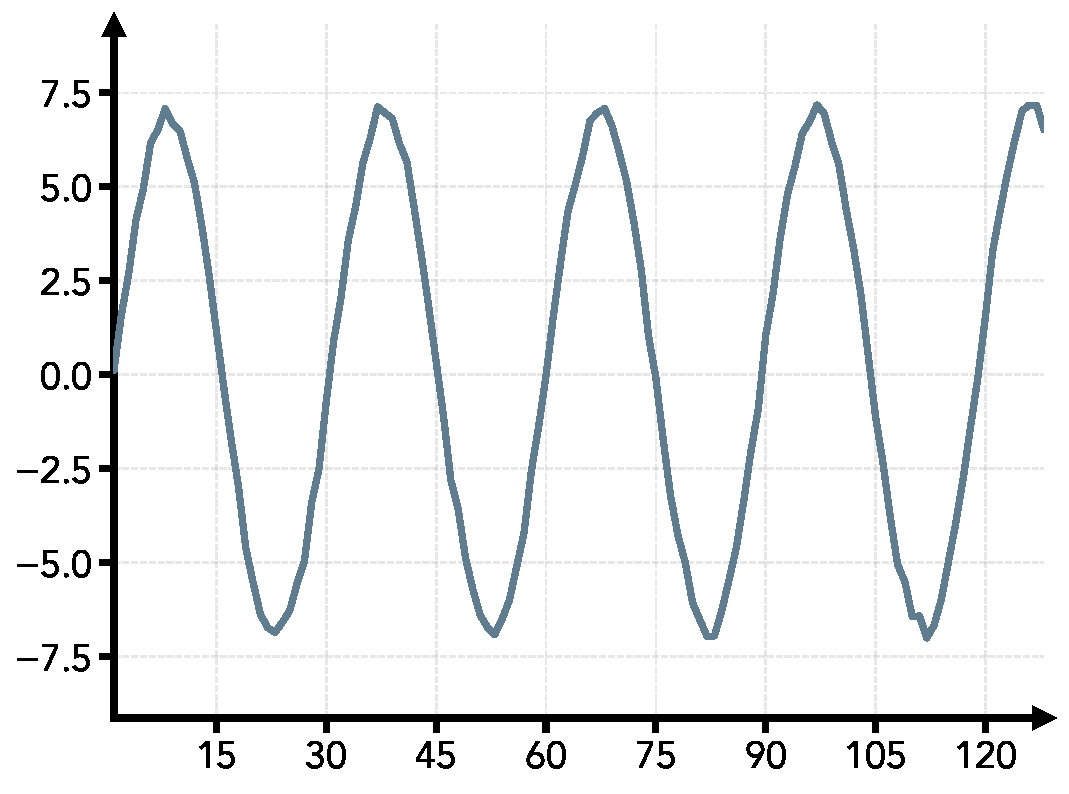
\includegraphics[width=\linewidth]{blocks/sample_cases_success/pattern.pdf}
        % 调整底部的留白
        \vspace{-20pt}
    \end{wrapfigure}
        \textbf{Question:} What is the most dominant pattern in this complex time series?

    \vspace{1.5em}

    % --- 第二部分：选项 ---
    \textbf{Answer Choices:} \\ (A) Noise \\ (B) Trend \\ (C) Seasonality \\
    \textbf{Correct Answer:} \textcolor{correctgreen}{(C)} \\
\end{ReasoningBox}